\chapter{Results}
\label{ch:results}

\emph{In this chapter the results of the experiments and methods detailed in the methodology chapter \Sref{ch:methodology} and background chapter \Sref{ch:background} are presented.}
\emph{A detailed analysis of the results is included along with references to similar results within the literature.}
\emph{Both quantitative and qualitative analysis is carried out and the limitations of the metrics used are discussed.}

\emph{First, the reproduction of steering clear \citep{steering-clear} detailed in \Sref{sec:steering-clear} is presented.}
\emph{Comparisons to the original paper are made along with additional analysis.}
\emph{This provides hypotheses about how the same adaptors will behave in the natural language setting of LLMs \Sref{sec:prompt-pairs}.}

\emph{Finally, the natural language setting described in the methodology chapter \Sref{sec:prompt-pairs} is analysed.}
\emph{A comparison to the steering clear toy environment is made focusing on the hypotheses proposed.}
\emph{Additionally, an in depth analysis of the hyperparameter choice in comparison to the toy environment is carried out.}
\emph{This provides potential further avenues of research and implications of superposition \Sref{sec:sae} on steering adaptors.}

\section{Steering Clear Reproduction}
\label{sec:steering-clear-res}

\begin{figure}
    \centering
    \captionsetup{width=\textwidth}
    \includegraphics[width=\textwidth]{figures/steering_clear.png}
    \caption{
        Reproduction of Figure 1 (top-left) in \citet{steering-clear}.
        Instead of overlaying all the data in a single plot the for methods are separated.
        ACE \citep{ace} is introduced and MiMiC \citep{mimic} is removed.
        Though the metric is different, focusing on the steered attribute rather than all attributes, the same trends are presents.
        The model accuracy is changed to reflect the accuracy of the model without steering rather than the model accuracy on the target input.
    }
    \label{fig:steering-clear}
\end{figure}

Following the experiment described in \Sref{sec:steering-clear} the results of \cite{steering-clear} are reproduced in \Fref{fig:steering-clear}.
There are a few changes from Figure 1 in \cite{steering-clear}, primarily the steering metric focuses on the steered attribute rather than entire output label.
Furthermore, affine concept editting (ACE) \citep{ace} is added and minimally modified counterfactuals (MiMiC) \citep{mimic} is removed.
A full discussion of the different metric and why this was used is presented in \Sref{app:steering-clear}.

\Fref{fig:steering-clear} only represents the upper-left plot in \cite{steering-clear} Figure 1.
This reproduction aims to verify the method used in \cite{steering-clear} and the results achieved as a stepping stone towards carrying out a similar analysis for large language models (LLMs).

The figure clearly shows a difference between the linear/affine methods of contrastive activation addition (CAA) \citep{caa} \& ACE and the low-rank methods of low-rank representation finetuning (LoReFT) \citep{reft} \& low-rank representation steering (LoReST) \citep{steering-clear}.
In the limit of more examples both low-rank methods achieve near 100\% success rate in steering the target attribute to the target value.
In comparison the affine methods reach an asymptote which does not increase with more training examples.
Importantly, in the low training example setting both LoReFT performs worse than both CAA and ACE.
In fact, it performs worse than the model without steering.
This is due to the requirement to train parameters which both affine approaches lack.
However, the addition of parameters allows the method to perform better as more examples are presented.
This feature of improvement with more examples is shared with LoReST.

Across the methods there is a critical hyperparameter above which the methods perform comparably.
In the case of CAA (in this environment) this appears to be $\lambda=2$.
For LoReFT the threshold rank is likely 3 as 2 decreases in accuracy as more examples are introduced.
Finally with LoReST the rank is clearly 2.
ACE behaves differently due to it's design (detailed in \Sref{sec:ace}) where the parameters relate to the strength of the behaviour more directly.
This is visible in \Fref{fig:steering-clear} as clear bands as the hyperparameter increases; in comparison to the other plots where after a threshold hyperparameter value the adaptors behave similarly.

Similar to the findings of \citet{steering-clear} LoReFT plateaus after 256 examples which coincides with the dimension of the activation space.
This distinction is not present in the other methods though this is similar to the Figure in \citet{steering-clear}.
A possible explanation for this in the case of the affine methods is they do not learn their own representation.
Instead, with sufficient opposing examples, the difference in steering direction is minimal with more examples.

LoReST in comparison to both LoReFT and the affine examples incorporates both approaches.
This means in the low data regime it likely behaves closer to ACE and CAA, then when enough data is provided that it can encode the concepts sufficiently the accuracy increases.
This is supported by the fact that LoReST achieves $\sim 0.8$ with 4 examples matching CAA, LoReST then continues to increase in accuracy following a similar arc to ACE eventually plateauing at the same values as LoReFT.
This behaviour is matched in \citet{steering-clear}.

Overall, the results suggest that the analysis by \citet{steering-clear} are sound though an exact replication was not achieved.
This also suggests some expectations for the prompt pairs environment (described in \Sref{sec:prompt-pairs}).
In particular
\begin{enumerate}[nolistsep]
    \item Affine methods will perform consistently across the number of examples used, though minor variation may occur.
    \item Low rank methods will increase with the number examples eventually plateauing.
    \item LoReST is likely to achieve the best performance.
\end{enumerate}

\section{Prompt Pairs}
\label{sec:prompt-pairs-res}

\subsection{Quantitative Analysis}

The three quantitative metrics discussed in \Sref{sec:prompt-pairs} can be split into two categories: the activation of the SAE features, the semantic similarity of the generated completions.
As there is no notion of accuracy akin to \citet{steering-clear} the closest comparison comes from the activation of SAE features.
Though the domains are different the same trends that were seen in \Sref{sec:steering-clear-res} should be seen in this new setting.

\subsubsection{SAE Feature Activation}

\begin{figure}
    \centering
    \captionsetup{width=\textwidth}
    \includegraphics[width=\textwidth]{figures/gpt2_7_target.png}
    \caption{
        The average activation of target SAE features at the model completion tokens.
        This represents how well the adaptor positively changed the models representation, \emph{higher} values are better.
        The y axis is a symmetric logarithm scale where the range $[0,1]$ is linear, this section is highlighted in grey.
        The same range of examples is used across all adaptors.
    }
    \label{fig:gpt-pp-target}
\end{figure}

\Fref{fig:gpt-pp-target} presents the results of the first metric, the average activation of the target SAE features.
As discussed in \Sref{sec:prompt-pairs} the target SAE features are the SAE features that had the highest, average activation across all positive examples.
For this reason, a successful adaptor should increase the activation of these SAE features from the model with no intervention.

The figure uses a symmetric logarithm plot so that the 4 methods can be compared across the same scale even though their SAE activations are orders of magnitude different.
The symmetric logarithm is used as the model achieves approximately 0 activation in instances which would cause issues with a standard log plot.
The linear region of the plot is highlighted in gray and a horizontal grid is provided to demonstrate the difference.

From the figure it is clear that all methods provide some level of improvement regardless of hyperparameter.
However, the results presented do not precisely follow those of \citet{steering-clear} or the hypotheses suggested in \Sref{sec:steering-clear-res}.
The primary outliers are affine concept editting (ACE) \citep{ace} and low-rank representation steering (LoReST) \citep{steering-clear}.

\smalltitle{contrastive activation addition (CAA) \citep{caa}} behaves according to the first hypothesis in \Sref{sec:steering-clear-res} and matches the behaviour in the steering clear environment \Sref{sec:steering-clear}.
There is a clear increase in effectiveness as the hyperparemeter increases and the performance is constant across the number examples with minor fluctuations.

In the case of $\lambda = 5$ the adaptor achieves an average SAE activation of $46.7 \pm 7.8$ across the range of training examples.
In the case of $\lambda = 1$ the adaptor achieves an average of $1.2 \pm 0.01$.
This demonstrates a very consistent value across the number of examples regardless of hyperparameter.
However, the larger the parameter the greater the variance in the exact SAE feature activation.

In comparison to CAA in \citet{steering-clear}, presented in \Fref{fig:steering-clear}, the same behaviour is observed.
A consistent value across the number of steering examples with a clear threshold above $\lambda = 1$.
This suggests that in unseen examples the CAA adaptor has to overcompensate and perturb the representation further in representation space than what was learnt.

\smalltitle{affine concept editting (ACE) \citep{ace}} does not behave as expected or in line with the findings presented in \Sref{sec:steering-clear-res}.
The hyperparameter does not change the target activation significantly and across trained examples the average activation value decreases.
The method, however, has the highest average target activation by an order of magnitude compared to the next best adaptor.
This is accompanied by the largest variance across the adaptors, at its best ACE achieves a feature activation of $2187$ but has a standard deviation of $2912$.
This variance is consistent across the range of training examples.
The problem of variability across all the adaptors is discussed further in \Sref{sec:variability}.

Given that \citet{ace} demonstrate impressive performance of ACE on Llama 3 \citep{llama3} and the comparable performance of ACE and CAA in \Fref{fig:steering-clear} it is likely that the task, the model or the metric are ill suited to the adaptor.
The immergent properties present in larger models such as Llama 3 \citep{llama3} and GPT 5 \citep{gpt-5} are not as prominent in the smaller GPT 2 \citep{gpt-2} model.
It is possible that across positive and negative examples there is not a clear, meaningful baseline from which ACE can consistently steer from.
This could be due to the completions involving free-text answers that have a range of interpretations that may not align with the desired interpretation.
\textcolor{red}{Ablation studies into this behaviour have not been carried out ... how easy would it be to do this?}

\smalltitle{Low-rank representation finetuning (LoReFT) \citep{reft}} behaves according to \citet{steering-clear} and the second hypothesis in \Sref{sec:steering-clear-res}. In particular there is a clear increase in target feature activation as the number of examples increases until a threshold point from which the adaptor does not improve.

In the majority of hyperparameter choices the best performance occurred between 128 and 512 examples.
This does not line up with the predictions of \citet{steering-clear} who found that the point of best performance occurred when the number of examples matched the activation dimension.
In \Fref{fig:gpt-pp-target} the activation dimension of GPT2 is 756 \citep{saelens} compared to the optimal performance occurring at 128-512 examples.

The key differences between the toy setup and this environment is the added complexity of superposition \Sref{sec:sae}.
However, this would suggest that superposition \emph{decreases} the number of required examples to successfully steer.
Another possibility is the rank of the adaptor is too small to accurately steer the model.
This is supported by the fact that the average feature activation decreases rather than plateaus similar to the small rank examples in \Fref{fig:steering-clear} (see $rank=1, 2$).
A deeper analysis of the role of the rank is discussed further in \Sref{sec:rank-res}.

LoReFT at its optimal is comparable to CAA achieving an average feature activation of $42.8 \pm 37.2$ in comparison to CAA with $49.3 \pm 26.3$.
However, in comparison to CAA, LoReFT requires careful tuning of the hyperparameter and the number of examples provided.
This behaviour is seen both in this realistic environment and the toy environment \Sref{sec:steering-clear-res}.

\smalltitle{Low-rank representation steering (LoReST) \citep{steering-clear}} does not behave as hypothesised in \Sref{sec:prompt-pairs-res} nor follow the trend presented in \citet{steering-clear}.
In comparison to \Fref{fig:steering-clear} there is no clear increase in the chosen metric as the number of examples increase.
Furthermore, the optimal rank appears to be $3$ rather than the larger ranks as anticipated.
Even the optimal rank of $3$ appears to perform worse that CAA with LoReST's average of $1.17 \pm 0.03$ compared to $1.21 \pm 0.01$ for CAA.

From \Fref{fig:steering-clear} it may be expected that the exact rank of LoReST has limited effect on the performance of the adaptor.
However, the results in \Fref{fig:steering-clear} suggest that there is a hyperparameter threshold above which the adaptor performs similarly \emph{but} higher values are not necessarily better.

\begin{figure}
    \centering
    \captionsetup{width=\textwidth}
    \includegraphics[width=\textwidth]{figures/gpt2_7_unrelated.png}
    \caption{
        The average activation of unrelated SAE features at the model completion tokens.
        This represents how well the adaptor did not interfere, \emph{lower} values are better.
        The y axis is a symmetric logarithm scale where the range $[0,1]$ is linear, this section is highlighted in grey.
        This demonstrates that all but ACE achieve 0 interference in some instances.
        The same range of examples is used across all adaptors.
    }
    \label{fig:gpt-pp-unrelated}
\end{figure}

Unlike the other adaptors presented here LoReST has not be thoroughly applied to large language models (LLMs).
It is possible that this approach, though based on adaptors such as LoReFT, is not suitable.
\emph{However}, as demonstrated in both \Fref{fig:gpt-pp-unrelated} and \Sref{sec:qual} the seemingly poor performance of LoReST suggests that feature activation alone is a poor metric for assessing success of a steering adaptor.

\subsubsection{The Importance of Rank}
\label{sec:rank-res}

\subsubsection{The Issue with Variability}
\label{sec:variability}

\subsubsection{Semantic Similarity}

\begin{figure}
    \centering
    \captionsetup{width=.9\textwidth}
    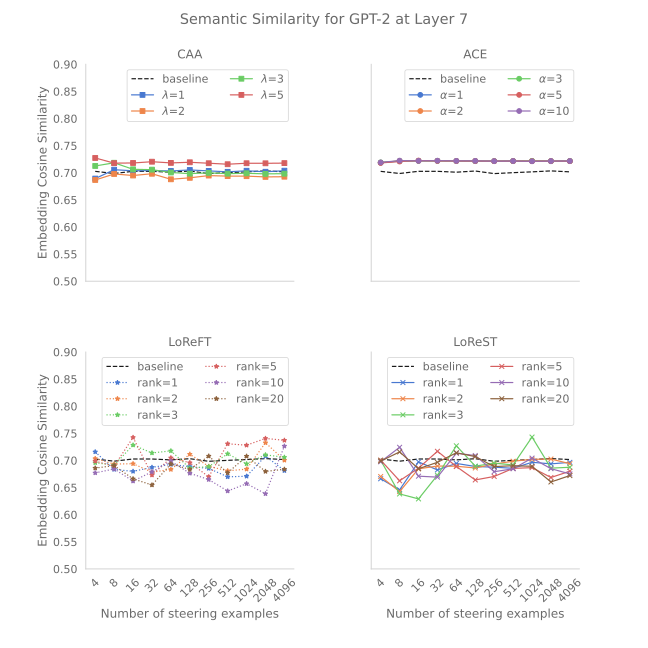
\includegraphics[width=\textwidth]{figures/gpt2_7_similarity.png}
    \caption{
        The cosine similarity of distilbert \citep{distilbert} sentence embeddings for the generated completion.
        The higher the cosine similarity the better the method has performed.
        The number of steering examples is the same as \Fref{fig:steering-clear} and the cosine similarity is shared across charts.
    }
    \label{fig:gpt-pp-sim}
\end{figure}

\subsection{Qualitative Analysis}
\label{sec:qual}
